\documentclass[border=10pt]{standalone}
\usepackage[svgnames]{xcolor}
\usepackage{amsmath}
\usepackage{pgfplots}
\pgfplotsset{compat=newest}
\usepackage[sfdefault]{FiraSans}
\usepackage{FiraMono}
\renewcommand*\familydefault{\sfdefault}
\begin{document}
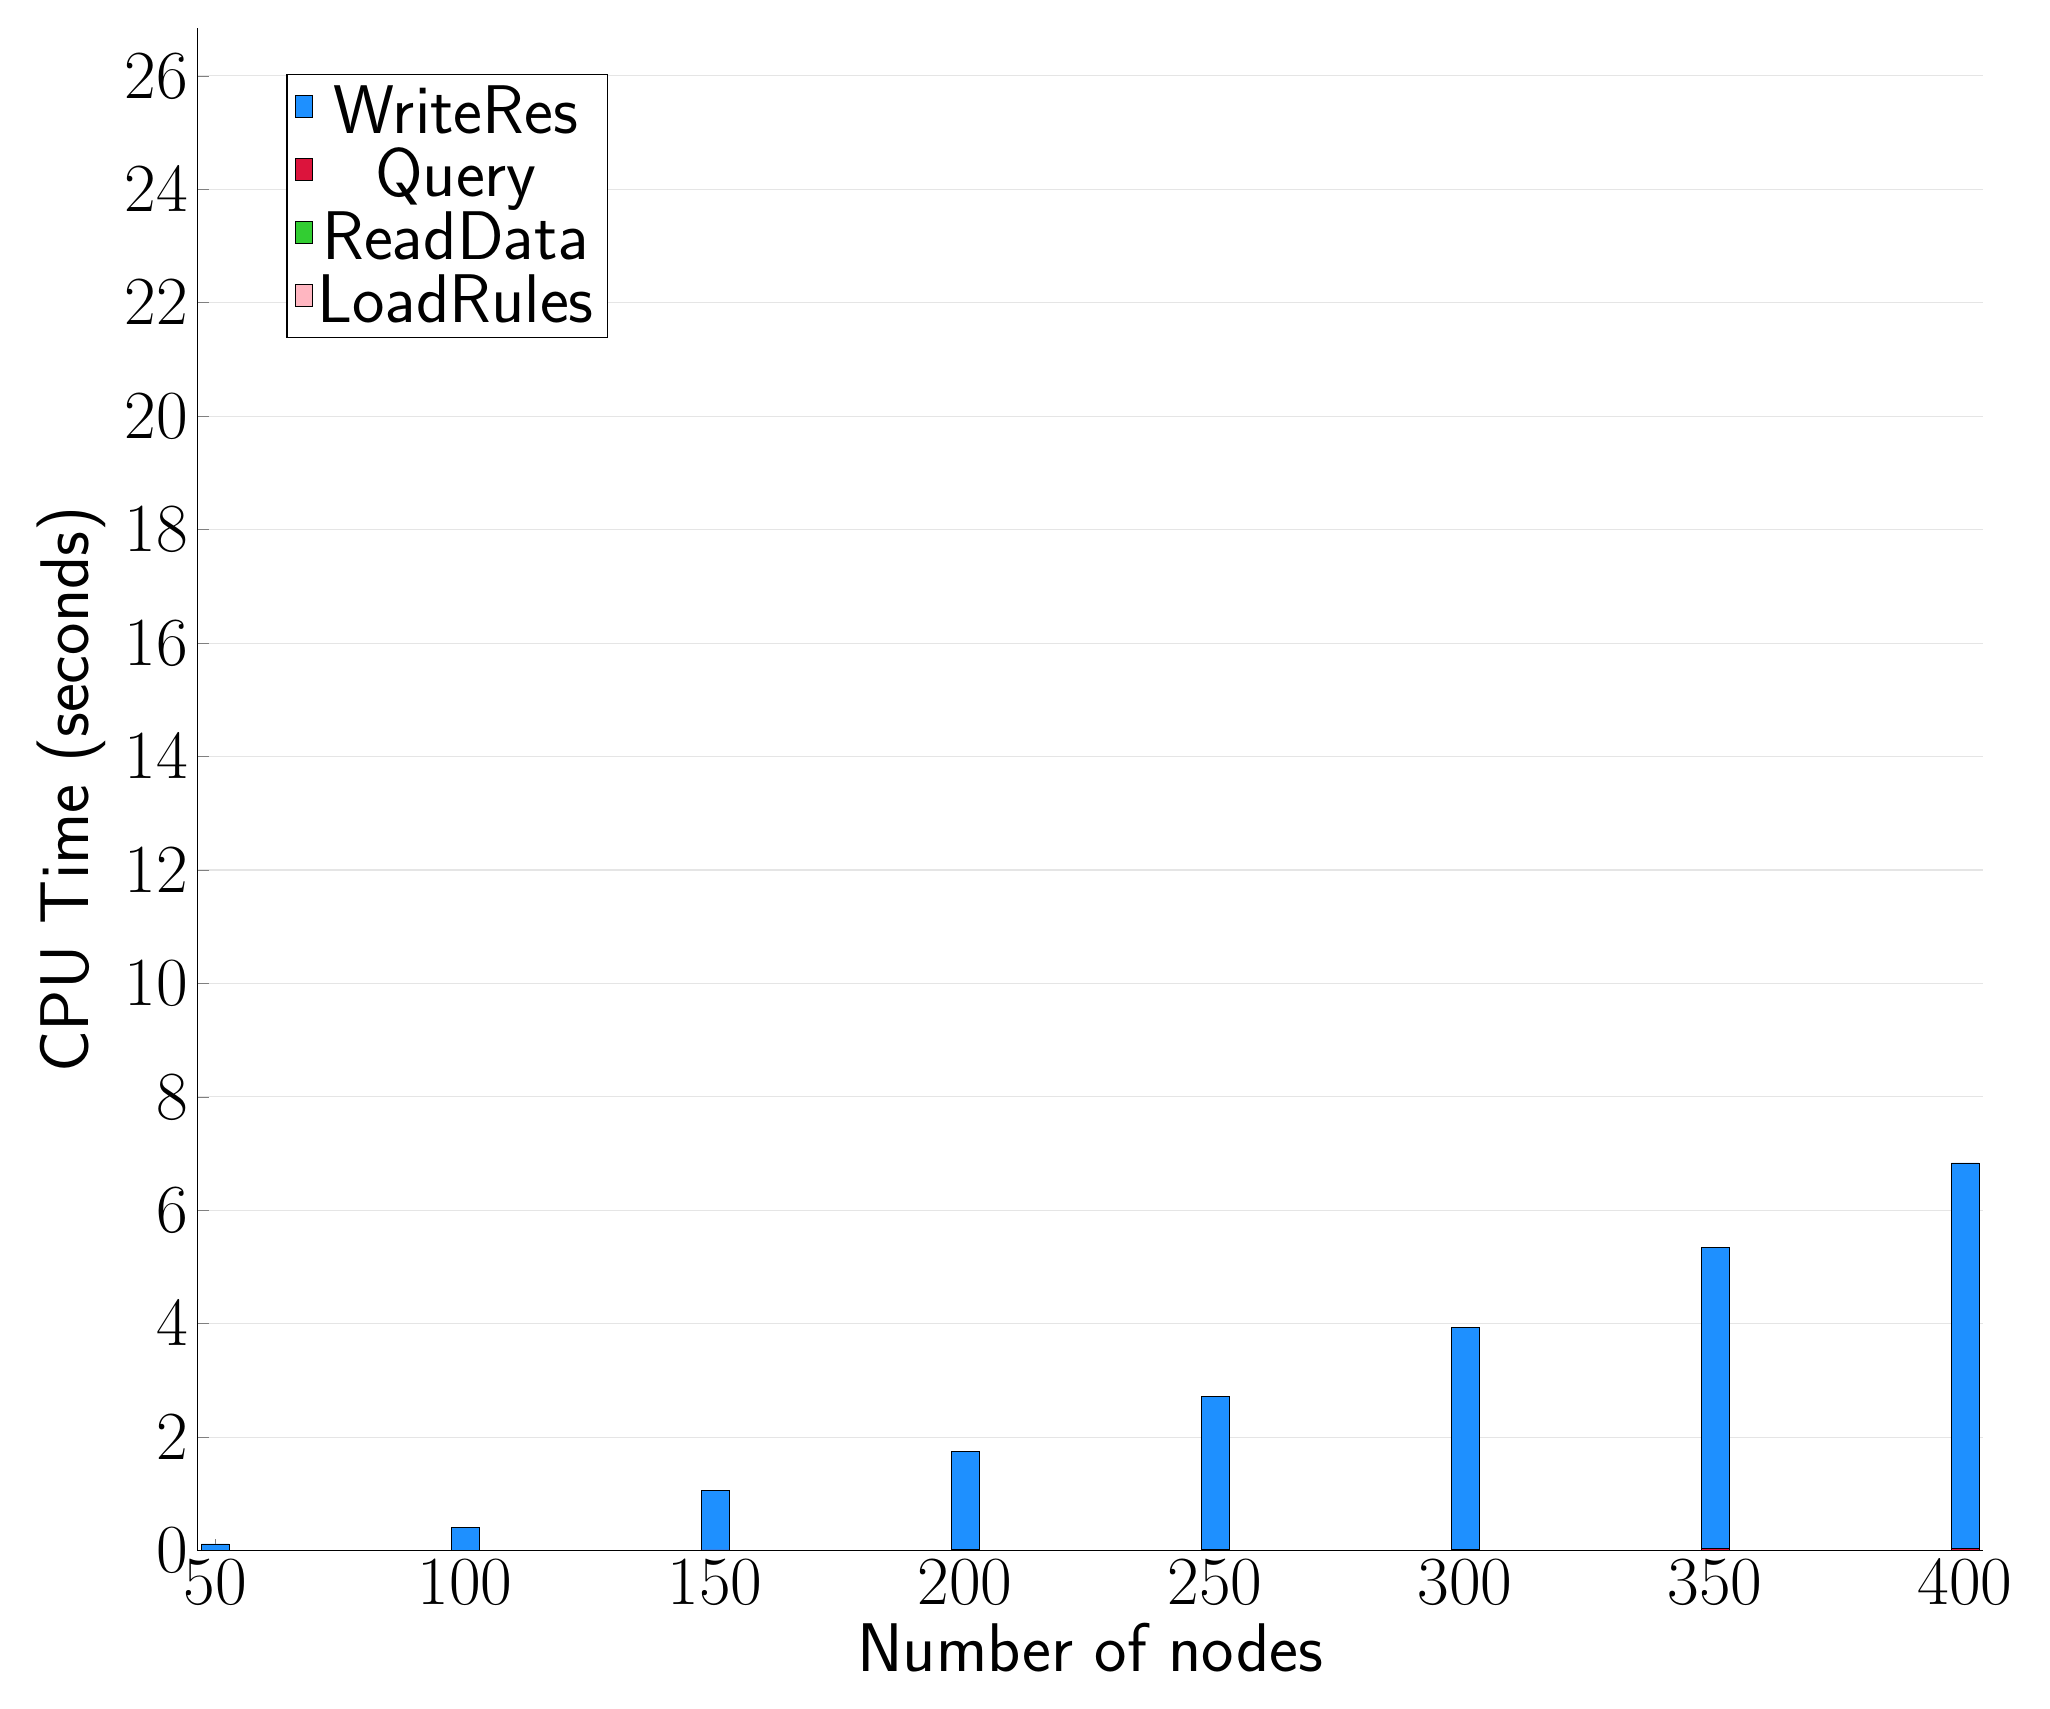
\begin{tikzpicture}
\begin{axis}[
   ybar stacked,
   width=2\textwidth,
   bar width=0.35cm,
   ymajorgrids, tick align=inside,
   major grid style={draw=gray!20},
   xtick=data,
   ymin=0, ymax=26.83928736050924,
   axis x line*=bottom,
   axis y line*=left,
   enlarge x limits=0.01,
   legend style={
       at={(0.23, 0.97)},
       anchor=north east,
       legend columns=1,
       font=\Huge,
   },
   ylabel={CPU Time (seconds)},
   xlabel={Number of nodes},
   label style={font=\Huge},
   tick label style={font=\Huge},
]
\addlegendimage{fill=DodgerBlue, draw=black, line width=0.2pt}
\addlegendentry{WriteRes}
\addlegendimage{fill=Crimson, draw=black, line width=0.2pt}
\addlegendentry{Query}
\addlegendimage{fill=LimeGreen, draw=black, line width=0.2pt}
\addlegendentry{ReadData}
\addlegendimage{fill=LightPink, draw=black, line width=0.2pt}
\addlegendentry{LoadRules}
\addplot +[fill=LightPink, draw=black, line width=0.2pt] coordinates {
(50, 0.005037)
(100, 0.0032913333333333358)
(150, 0.00409933333333333)
(200, 0.003981333333333333)
(250, 0.004285333333333333)
(300, 0.0028359999999999995)
(350, 0.005168)
(400, 0.004040666666666667)
};
\addplot +[fill=LimeGreen, draw=black, line width=0.2pt] coordinates {
(50, 0.0017973333333333333)
(100, 0.00161733333333333)
(150, 0.0029876666666666667)
(200, 0.003465666666666667)
(250, 0.004220333333333333)
(300, 0.0028613333333333334)
(350, 0.00570166666666667)
(400, 0.006560666666666666)
};
\addplot +[fill=Crimson, draw=black, line width=0.2pt] coordinates {
(50, 0.0008396666666666643)
(100, 0.002362)
(150, 0.008035333333333337)
(200, 0.011458000000000001)
(250, 0.013287666666666665)
(300, 0.022194333333333333)
(350, 0.032025)
(400, 0.034131666666666664)
};
\addplot +[fill=DodgerBlue, draw=black, line width=0.2pt] coordinates {
(50, 0.11081400000000001)
(100, 0.40663000000000005)
(150, 1.052831)
(200, 1.7317893333333334)
(250, 2.700089333333333)
(300, 3.902504)
(350, 5.308592333333333)
(400, 6.7920343333333335)
};
\end{axis}
\end{tikzpicture}

\end{document}
